\documentclass[a4paper,11pt]{article}
\input{/home/tof/Documents/Cozy/latex-include/preambule_lua.tex}
\newcommand{\showprof}{show them}  % comment this line if you don't want to see todo environment
\fancyhead[L]{Exercices supplémentaires 2}
\newdate{madate}{10}{09}{2020}
%\fancyhead[R]{\displaydate{madate}} %\today
%\fancyhead[R]{Seconde - SNT}
\fancyhead[R]{Première - NSI}
%fancyhead[R]{Terminale - NSI}
\fancyfoot[L]{~\\Christophe Viroulaud}
\AtEndDocument{\label{lastpage}}
\fancyfoot[C]{\textbf{Page \thepage/\pageref{lastpage}}}
\fancyfoot[R]{\includegraphics[width=2cm,align=t]{/home/tof/Documents/Cozy/latex-include/cc.png}}

\begin{document}
\begin{Form}
\begin{exo}
On définit la suite $U_n$ par:
$$
U_n = \left\{
    \begin{array}{ll}
        3 & \mbox{si  n = 0}\\
        5*U_{n-1} + 4 & sinon\\
    \end{array}
\right.
$$
Écrire un programme qui demande un entier \emph{n} et qui calcule la valeur de $U_n$ correspondante.
\end{exo}
\begin{exo}
Écrire un programme qui demande un nombre de lignes et qui produit la construction suivante.

\begin{figure}[!h]
\centering
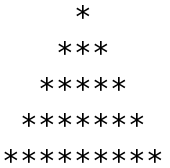
\includegraphics[width=5cm]{ressources/etoile.png}
\captionof{figure}{Exemple pour n = 5}
\label{etoile}
\end{figure}

\textbf{Aide:} Il est possible d'écrire plusieurs fois le même caractère avec le code \ref{repetition}
\begin{code}[!h]
\begin{lstlisting}
print(5*"a")
\end{lstlisting}
\captionof{code}{Écrire 5 fois la lettre \emph{a}}
\label{repetition}
\end{code}
\end{exo}
\end{Form}
\end{document}